% Capítulo 8. Resultados y análisis (rúbrica 50 pts).

Este capítulo presenta el plan del método para los tres tipos de día, explica de dónde sale el ahorro, justifica la elección de cuartetos al azar y mide qué tan cerca del óptimo queda la solución. Salvo que se diga otra cosa, el plan es el de cuartetos al azar con \MinutosFinal{} minutos de búsqueda por tipo de día y las cifras son el promedio de \SemillasPlanLaboral{} semillas.

\section{Resultado principal}
\label{sec:resultado-principal}

La Tabla~\ref{tab:resultado} compara el plan con el caso base. En día laboral, el plan cubre las mismas \CorridasLaboral{} corridas con \BusesPlanLaboral{} buses, \AhorroBusesLaboral{} menos que el caso base (\DeltaPctBusesLaboral\,\%), y cuesta USD~\CostoPlanLaboral{} al día, USD~\AhorroCostoLaboral{} menos (\DeltaPctCostoLaboral\,\%). El sábado y el domingo la reducción de buses es incluso mayor, \BajaBusesSabado{} y \BajaBusesDomingo\,\%. Si la semana se cuenta como cinco días laborales más un sábado y un domingo, el costo semanal pasa de USD~\CostoSemanaBaseMillones{} a \CostoSemanaPlanMillones{} millones, \BajaSemana\,\% menos. La flota que RED tendría que tener es la del día laboral, porque los otros días se cubren con una parte de ella.

\begin{table}[htbp]
\centering
\caption{Caso base y plan de cuartetos al azar en la red completa (promedio de tres semillas).}
\label{tab:resultado}
\small
\begin{tabular}{@{}lrrrrrr@{}}
\toprule
 & & \multicolumn{2}{c}{Buses} & \multicolumn{2}{c}{Costo (USD/día)} & \\
\cmidrule(lr){3-4}\cmidrule(lr){5-6}
Día & Corridas & Caso base & Plan & Caso base & Plan & $\Delta$ costo \\
\midrule
Laboral & \CorridasLaboral & \BusesBaseLaboral & \BusesPlanLaboral & \CostoBaseLaboral & \CostoPlanLaboral & \DeltaPctCostoLaboral\,\% \\
Sábado & \CorridasSabado & \BusesBaseSabado & \BusesPlanSabado & \CostoBaseSabado & \CostoPlanSabado & \DeltaPctCostoSabado\,\% \\
Domingo & \CorridasDomingo & \BusesBaseDomingo & \BusesPlanDomingo & \CostoBaseDomingo & \CostoPlanDomingo & \DeltaPctCostoDomingo\,\% \\
\midrule
Semana & & & & \CostoSemanaBase & \CostoSemanaPlan & \DeltaPctSemana\,\% \\
\bottomrule
\end{tabular}
\fuente{Plan en \texttt{09-entrega3/octetos/resultados/red\_completa\_417\_\{L,S,D\}.csv} y caso base en \texttt{09-entrega3/kpi/resultados/kpi\_planes.csv}. La semana suma cinco días laborales, un sábado y un domingo.}
\end{table}

\section{De dónde sale el ahorro}
\label{sec:origen-ahorro}

La Tabla~\ref{tab:pasos} sigue el día laboral paso a paso. El plan inicial, que todavía no optimiza nada, ya baja la flota de \BusesBaseLaboral{} a \BusesInicialLaboral{} buses (\DeltaPctBusesInicialLaboral\,\%). Así, el \PctAhorroInicial\,\% de la reducción total viene de compartir buses entre las rutas de un sector, de cargar solo lo necesario y de elegir el bus que queda más cerca, y no de la búsqueda. La mejora por grupos agrega el resto. Con pares y tríos, el método de la Entrega~2, llega a \BusesMetodoParesTrios{} buses, y con cuartetos al azar a \BusesPlanLaboral, \MejoraInicialLaboral\,\% de costo sobre el plan inicial. En sábado y domingo la búsqueda aporta más, \MejoraInicialSabado{} y \MejoraInicialDomingo\,\%, porque esos días los buses cargan más y la búsqueda tiene más recargas que reorganizar.

\begin{table}[htbp]
\centering
\caption{Buses y costo del día laboral en cada etapa.}
\label{tab:pasos}
\small
\begin{tabular}{@{}lrrr@{}}
\toprule
Etapa & Buses & Costo (USD/día) & $\Delta$ costo contra el caso base \\
\midrule
Caso base miope & \BusesBaseLaboral & \CostoBaseLaboral & --- \\
Plan inicial del método & \BusesInicialLaboral & \CostoInicialLaboral & \DeltaPctCostoInicialLaboral\,\% \\
Mejora por pares y tríos, \MinutosFinal{} min & \BusesMetodoParesTrios & \CostoMetodoParesTrios & \\
Mejora por cuartetos al azar, \MinutosFinal{} min & \BusesPlanLaboral & \CostoPlanLaboral & \DeltaPctCostoLaboral\,\% \\
\bottomrule
\end{tabular}
\end{table}

Por componente, cerca de tres de cada cuatro dólares ahorrados son buses (Figura~\ref{fig:ahorro}). Los buses aportan USD~\AhorroCompFlota{} diarios, el \PctAhorroCompFlota\,\% del ahorro, la energía USD~\AhorroCompEnergia{} y los kilómetros USD~\AhorroCompKm. Los kilómetros en vacío bajan \BajaVacioLaboral\,\%, de \PctVacioBaseLaboral{} a \PctVacioPlanLaboral\,\% de los kilómetros totales, porque un bus puede encadenar corridas de distintas rutas que empiezan cerca de donde terminó. Cada bus del plan hace \CorridasPorBusPlanLaboral{} corridas en promedio, contra \CorridasPorBusBaseLaboral{} en el caso base.

\begin{figure}[htbp]
\centering
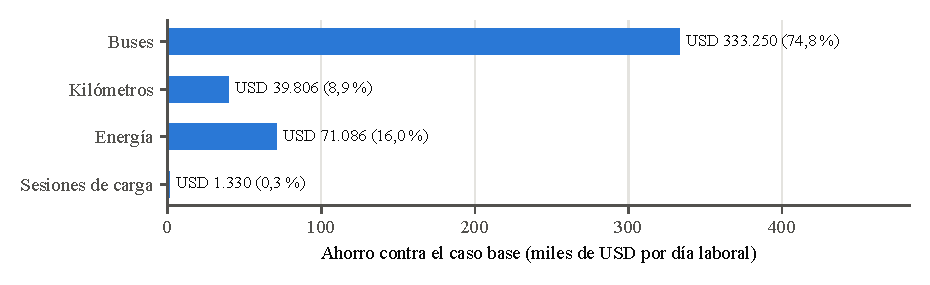
\includegraphics[width=\textwidth]{figures/ahorro_componentes.pdf}
\caption{Ahorro diario del plan frente al caso base por componente del costo, día laboral.}
\label{fig:ahorro}
\end{figure}

\section{Uso de los electroterminales y de la energía}
\label{sec:uso-e}

La Figura~\ref{fig:uso-e} muestra cuántos buses cargan a la vez durante el día laboral en toda la red. El caso base concentra la carga al anochecer y llega a \PicoCargandoBase{} buses cargando a la vez en El Conquistador a las \HoraPicoCargandoBase, con \ElectroterminalesLlenosBase{} electroterminales con todas sus conexiones ocupadas. El plan, en cambio, nunca pasa de \PicoCargandoPlan{} buses cargando a la vez en un electroterminal, entre el \PctConexionesMinPlan{} y el \PctConexionesMaxPlan\,\% de sus conexiones, con el máximo entre las \HoraPicoMinPlan{} y las \HoraPicoMaxPlan. Durante el día los cargadores no son un cuello de botella. El sábado el uso sube, y en \PctConexionesMaxEPlanSabado{} llega al \PctConexionesMaxPlanSabado\,\% de las conexiones.

\begin{figure}[htbp]
\centering
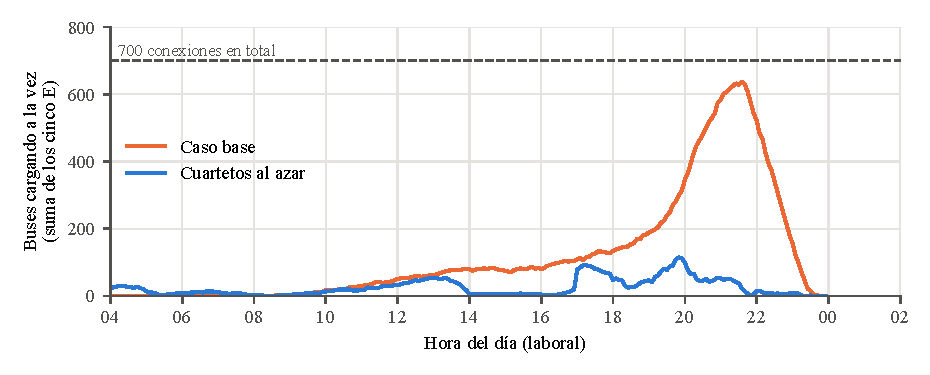
\includegraphics[width=\textwidth]{figures/uso_electroterminales.pdf}
\caption{Buses cargando a la vez en los cinco electroterminales, día laboral.}
\label{fig:uso-e}
\end{figure}

El plan carga muy poca energía durante el día. Los buses parten llenos, la mayoría alcanza a terminar su jornada sin cargar y la energía cargada es \BajaEnergiaCargadaLaboral\,\% menor que en el caso base, apenas el \PctEnergiaCargadaPlanLaboral\,\% de la que se consume. Por eso la energía pesa solo el \PctEnergiaPlanLaboral\,\% del costo del plan. La Figura~\ref{fig:energia-hora} muestra en qué horario se carga, que fue una de las preguntas de la Entrega~2. La mitad de la energía del plan, el \PctEnergiaPuntaPlan\,\%, cae en los tramos de tarifa más alta, contra el \PctEnergiaPuntaBase\,\% del caso base, y la hora en que más carga el plan es de \HoraMasCargaPlan{} a \HoraMasCargaFinPlan{} horas. El plan carga lo justo para terminar sus corridas y lo hace cuando los buses lo necesitan, y en promedio paga USD~\PrecioMedioKwhPlanLaboral{} por kWh, contra \PrecioMedioKwhBaseLaboral{} del caso base. Mover esa carga a horas más baratas casi no cambiaría el costo total, como confirma la sensibilidad a la tarifa (sección~\ref{sec:sens-capacidad}).

\begin{figure}[htbp]
\centering
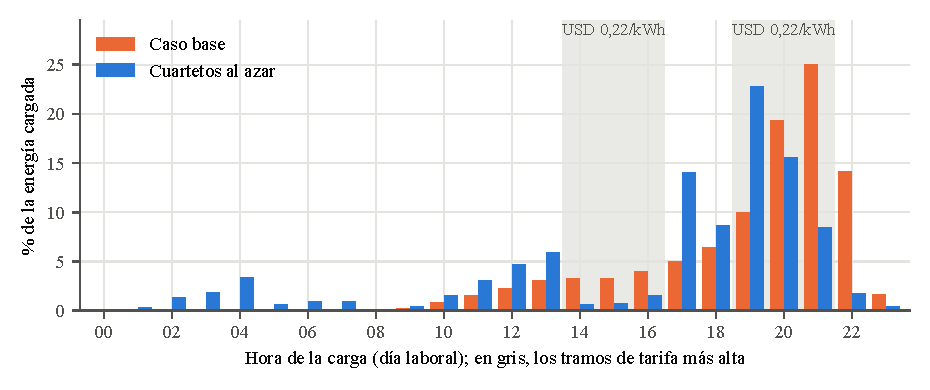
\includegraphics[width=\textwidth]{figures/energia_hora.pdf}
\caption{Distribución horaria de la energía cargada en el día laboral, como porcentaje de lo que carga cada plan.}
\label{fig:energia-hora}
\end{figure}

Las plazas tampoco limitan durante la operación. En el día laboral la ocupación máxima va del \PctPlazasOperacionMin{} al \PctPlazasOperacionMax\,\% de las plazas de cada electroterminal. Se llenan solo al cierre, cuando \BusesTerminanEPlanLaboral{} buses del plan terminan el día estacionados en los electroterminales, y pasada la medianoche permanecen completos entre \MinutosPlazasLlenasMin{} y \MinutosPlazasLlenasMax{} minutos. Ese uso de las plazas al cierre importa para la recarga nocturna, que se analiza en la sección~\ref{sec:repetibilidad}.

La Tabla~\ref{tab:sectores} muestra el plan por sector. El ahorro es parejo, entre 14 y 17\,\% de los buses en cada sector, así que ningún sector concentra la ganancia. Lo que no es parejo es dónde se carga. Los sectores cargan entre el \PctCargaPropiaOtrosMin{} y el \PctCargaPropiaOtrosMax\,\% de su energía en su propio electroterminal, salvo Los Espinos, que carga solo el \PctCargaPropiaTres\,\% en el suyo y el \PctEspinosEnDos\,\% en El Conquistador. Que sus buses puedan cargar donde les queda más a mano es una ventaja de no atar la carga al sector.

\begin{table}[htbp]
\centering
\caption{Plan del día laboral por sector.}
\label{tab:sectores}
\small
\begin{tabular}{@{}lrrrrrr@{}}
\toprule
Sector & Rutas & Corridas & Buses caso base & Buses plan & $\Delta$ buses (\%) & Carga en su E (\%) \\
\midrule
\tabla{sectores}
\bottomrule
\end{tabular}
\fuente{\texttt{09-entrega3/kpi/resultados/kpi\_por\_sector.csv}, plan de cuartetos con semilla 1.}
\end{table}

\section{Elección del método}
\label{sec:metodo-elegido}

La Tabla~\ref{tab:metodos} compara todas las variantes de la mejora en el día laboral con 10, 20 y 40 minutos de búsqueda. La regla fue quedarse con la más barata a igual tiempo, y cuartetos al azar gana con los tres tiempos. La Figura~\ref{fig:tamano} resume el efecto del tamaño del grupo. Con tres buses por grupo cada propuesta es barata, pero hay pocas formas de repartir las corridas; con ocho hay muchas, pero cada intento tarda tanto que en el mismo tiempo se prueban muy pocos. Cuatro buses queda en el punto intermedio de ese dilema \cite{ahuja_vlsn_2002}. La segunda lectura es que elegir los buses al azar le gana a elegirlos por horarios parecidos con cualquier tamaño de grupo. Los grupos parecidos se repiten, la búsqueda queda atrapada en las mismas combinaciones y deja de mejorar antes de agotar el tiempo, como pasa con cuartetos parecidos, que se queda en \BusesMetodoCuartetosParecidos{} buses.

\begin{table}[htbp]
\centering
\caption{Buses del plan del día laboral según la variante de la mejora y el tiempo de búsqueda. Las variantes al azar son el promedio de tres semillas.}
\label{tab:metodos}
\small
\begin{tabular}{@{}lrrrrr@{}}
\toprule
 & \multicolumn{3}{c}{Buses según tiempo de búsqueda} & Costo (USD/día) & \\
\cmidrule(lr){2-4}
Variante & 10 min & 20 min & 40 min & con 40 min & Semillas \\
\midrule
\tabla{metodos_red}
\bottomrule
\end{tabular}
\fuente{\texttt{09-entrega3/octetos/resultados/red\_completa\_417\_L.csv}.}
\end{table}

\begin{figure}[htbp]
\centering
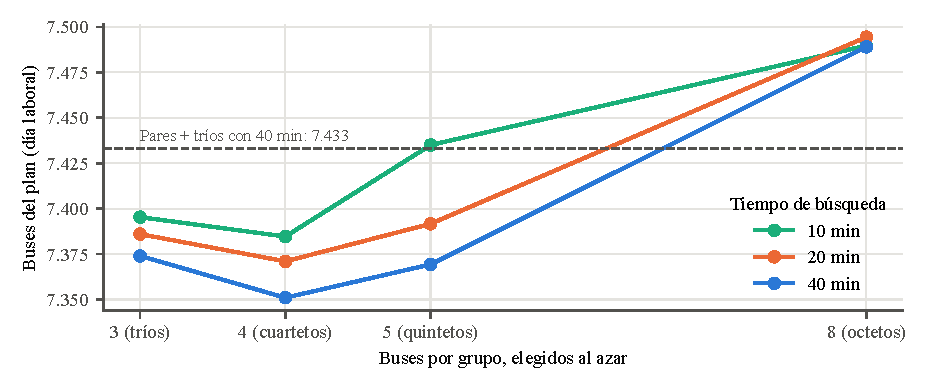
\includegraphics[width=\textwidth]{figures/tamano_grupo.pdf}
\caption{Buses del plan del día laboral según el número de buses por grupo, con selección al azar y tres tiempos de búsqueda.}
\label{fig:tamano}
\end{figure}

\section{Variabilidad de la búsqueda}
\label{sec:variabilidad}

La búsqueda depende de la semilla que fija el sorteo de los grupos. Con \MinutosFinal{} minutos, las tres semillas del día laboral dan entre \BusesSemillaMinLaboral{} y \BusesSemillaMaxLaboral{} buses, entre \BusesSemillaMinSabado{} y \BusesSemillaMaxSabado{} el sábado y entre \BusesSemillaMinDomingo{} y \BusesSemillaMaxDomingo{} el domingo. Con 20 minutos el costo de las tres semillas varía \RuidoSemillas\,\%. Esa dispersión es pequeña frente al ahorro contra el caso base, pero no frente a algunos efectos de la sensibilidad, y por eso se usa como banda de ruido en el capítulo~\ref{ch:sensibilidad}. La búsqueda también depende del reloj y del equipo, de modo que todos los métodos se compararon con el mismo tiempo y en el mismo computador.

\section{Calidad de la solución}
\label{sec:calidad}

El método no garantiza el óptimo, así que su calidad se midió de tres maneras.

La primera usa \CasosChicos{} casos chicos de 2 a 4 rutas, con \CorridasChicosMin{} a \CorridasChicosMax{} corridas, que el modelo exacto resolvió con óptimo demostrado en \MinutosExactaMin{} a \MinutosExactaMax{} minutos cada uno. La Tabla~\ref{tab:brecha-chicos} muestra la brecha de cada variante con \SegundosChicos{} segundos de búsqueda. El plan inicial queda en promedio a \BrechaInicial\,\% del óptimo, pares y tríos a \BrechaParesTrios\,\% y cuartetos al azar a \BrechaCuartetos\,\%, con un peor caso de \BrechaPeorCuartetos\,\%.

\begin{table}[htbp]
\centering
\caption{Brecha al óptimo en los cinco casos chicos, con 120 segundos de búsqueda. Las variantes al azar promedian tres semillas por caso, y el peor caso es la peor corrida individual.}
\label{tab:brecha-chicos}
\small
\begin{tabular}{@{}lrr@{}}
\toprule
Variante & Brecha media (\%) & Peor caso (\%) \\
\midrule
\tabla{brecha_chicos}
\bottomrule
\end{tabular}
\fuente{\texttt{09-entrega3/octetos/resultados/casos\_chicos.csv} y \texttt{casos\_chicos\_exacta.csv}.}
\end{table}

La segunda usa casos medianos, de 6 a 12 rutas, que se resolvieron con el modelo podado (Tabla~\ref{tab:casos-rutas}). Con 5 minutos y una semilla, cuartetos queda a menos de 1\,\% del óptimo en tres de los cuatro casos con óptimo, incluido el de \CorridasRutasDiez{} corridas, donde usa los mismos \BusesOptRutasDiez{} buses del óptimo. En el caso de 8 rutas queda a \BrechaCuartetosRutasOchoAbs\,\% con \BusesCuartetosRutasOcho{} buses contra \BusesOptRutasOcho{}, y ahí pares y tríos lo hace mejor. Ningún tamaño de grupo gana en todos los casos, y la brecha no crece con el número de corridas. En el caso de 12 rutas el modelo exacto se interrumpió a los 34 minutos y no hay óptimo.

\begin{table}[htbp]
\centering
\caption{Casos medianos con la batería del enunciado. Óptimo en buses y USD por día; las heurísticas usan 5 minutos y una semilla y se expresan en \% sobre el óptimo, con sus buses entre paréntesis. En 12 rutas el porcentaje es contra el plan inicial.}
\label{tab:casos-rutas}
\small
\begin{tabular}{@{}lrlrrr@{}}
\toprule
Caso & Corridas & Óptimo & Plan inicial & Pares + tríos & Cuartetos \\
\midrule
\tabla{casos_rutas}
\bottomrule
\end{tabular}
\fuente{\texttt{09-entrega3/octetos/resultados/casos\_rutas*.csv} y \texttt{casos\_medianos*.csv}.}
\end{table}

La tercera obliga a recargar. Con la batería de \Bateria~kWh casi ningún bus de estos casos necesita cargar, de modo que los casos anteriores prueban poco la parte de recarga del método. En las copias con baterías de 150 y 120~kWh (Tabla~\ref{tab:recarga-forzada}) la mejor heurística reduce el costo del plan inicial entre \MejoraRecargaMinCientoCincuenta{} y \MejoraRecargaMaxCientoCincuenta\,\% con 150~kWh y entre \MejoraRecargaMinCientoVeinte{} y \MejoraRecargaMaxCientoVeinte\,\% con 120~kWh. Con recarga, el exacto ya no demuestra el óptimo en 15 minutos, y su mejor plan queda entre \BrechaCotaRecargaMinCientoCincuenta{} y \BrechaCotaRecargaMaxCientoCincuenta\,\% sobre su propia cota. Contra ese mejor plan, que no es el óptimo, la heurística queda en promedio un \DifMediaRecargaCientoCincuentaAbs\,\% más cara con 150~kWh y un \DifMediaRecargaCientoVeinteAbs\,\% con 120~kWh, casi siempre por uno a cuatro buses más. En el caso más grande, de \CorridasGrande{} corridas, la heurística encuentra un plan con \BusesHeurGrande{} buses y USD~\CostoHeurGrande, mejor que el que encontró el exacto en una hora (\BusesExactaGrande{} buses y USD~\CostoExactaGrande). Darle 15 minutos a la heurística en vez de 2 casi no cambia el resultado, porque la búsqueda se detiene sola al no encontrar mejoras. El límite está en las operaciones que prueba y no en el tiempo, y la extensión natural es un movimiento que traspase recargas entre buses.

\begin{table}[htbp]
\centering
\caption{Recarga forzada. Mejor plan del exacto en 15 minutos (una hora en 10 rutas) y mejor heurística con 2 o 15 minutos.}
\label{tab:recarga-forzada}
\footnotesize
\resizebox{\textwidth}{!}{%
\begin{tabular}{@{}rlrrlrlr@{}}
\toprule
 & & & Buses plan & Exacto & Exacto sobre & Heurística & Heurística \\
kWh & Caso & Corridas & inicial & (buses · USD) & su cota (\%) & (buses · USD) & vs exacto (\%) \\
\midrule
\tabla{recarga_forzada}
\bottomrule
\end{tabular}}
\fuente{\texttt{09-entrega3/octetos/resultados/recarga\_bat150*.csv} y \texttt{recarga\_bat120*.csv}.}
\end{table}

En la red completa no hay óptimo, pero sí una cota. Ningún plan puede usar menos buses que las \SimultaneidadLaboral{} corridas en curso a la vez a las \HoraSimultaneidadLaboral{} ni recorrer menos que los kilómetros de servicio, lo que da un piso de USD~\CotaCosto{} al día. El plan queda \BrechaCotaCosto\,\% sobre ese piso en costo y \BrechaCotaBuses\,\% en buses. Es una cota débil, porque ignora la batería, los traslados en vacío y los sectores, de modo que la distancia real al óptimo es menor que esa cifra, aunque no se sabe cuánto.

Con estas tres mediciones la conclusión es que la solución es aproximada y no óptima. En los casos donde el óptimo se puede calcular queda en general a menos de 1\,\%, pero puede llegar a cerca de 5\,\% en algunos casos y con recarga forzada, y en la red completa solo se puede acotar.

\section{Relación con los objetivos}
\label{sec:relacion-objetivos}

El objetivo era un plan factible para toda la red y los tres tipos de día al menor costo posible, y se cumplió en sus tres partes. El plan cubre todas las corridas y pasó el auditor, y reduce el costo frente a una referencia razonable en los tres días. La reducción viene de lo que se esperaba atacar, el tamaño de la flota, y la calidad de la solución quedó medida contra el óptimo. Los dos aprendizajes que no se anticiparon al comenzar son que la mayor parte del ahorro la entrega una buena construcción y no la búsqueda, y que durante el día la infraestructura de carga sobra mientras que de noche falta, que es el tema del capítulo siguiente.
